\chapter{The Nature of LAPD Turbulence}
\label{c_lapd_turb}

Simulations can supplement experiment by providing detailed spatial data that is too difficult to obtain experimentally. This spatial data can be analyzed, revealing new properties
of the experiment. In order for simulations to provide information, however, they must accurately represent the system which they model. Assessing the validity of simulations generally
comes in two parts: verification and validation. Verification, the evidence that the code solves the equations correctly, will not be taken up here. I note, however, that my collaborators and I
have done verification studies in the past, somewhat detailed in Popovich et al.~\cite{Popovich2010a}. We compared linear BOUT (the old version of BOUT++) and BOUT++ simulations
to analytic solutions as well as to eigensystem solver solutions. On the other hand, I will focus parts of this chapter on our validation effort. Validation is the evidence that
the simulation model accurately reproduces features of the experiment. Generally, the more features of the experiment that the model reproduces, the more valid the model. While this chapter
focuses on simple analyses to describe the nature of the simulated turbulence, it will also make comparisons, where possible, to experimental data in order to show that the model is
relatively well validated. First, however, I analyze the linear instabilities in the LAPD simulations, and this affords no experimental comparison.

\section{LAPD Linear Instabilities}
\label{s_lin_inst}

Linear instabilities are prevalent in plasma physics. They come from the linearization around an equilibrium of the plasma equations. Physically, if a plasma is in a time-independent
steady state that is linearly unstable and a finite fluctuation of any size occurs, the fluctuation will grow exponentially. Linear instabilities often drive hydrodynamic and plasma
turbulence. I therefore study the linear instabilities of the LAPD system before moving onto the turbulence because they can offer insight into the nature of the turbulence.
The LAPD equations, parameters, and profiles described in Chapter~\ref{c_lapd_sim} give rise to a couple of linear instabilities. They are both drift wave type instabilities, but they 
have different pressure/potential coupling mechanisms. One type couples through the adiabatic response, while the other couples through the sheath boundary response.

\subsection{Drift Waves}
\label{ss_drift_waves}

Electron drift waves driven by an equilibrium density or pressure gradient that use the adiabatic response are generally referred to as just drift waves or the universal instability.
The electron drift wave mechanism is the following: An electron pressure fluctuation in the plasma is linked with a potential fluctuation through the adiabatic response. The adiabatic
response is simply a parallel force balance between the pressure force and the electrostatic force. A simplified version of Eq.~\ref{brag_mom} can be written:

\beq
\label{adiabatic_response}
\gradpar p_e = e n \gradpar \phi + R \vpe,
\eeq

where the term $R \vpe$ represents effects such as electron inertia, resistivity, and electromagnetic induction. If $R=0$, the electrons are said to be adiabatic, meaning 
$\gradpar p_e = e n \gradpar \phi$. When $T_e$ fluctuations are neglected and $\gradpar \ne 0$, this integrates to the Boltzmann expression:

\beq
\label{boltzmann_exp}
n = n_0 e^{e \phi/T_e}.
\eeq

For any $R$ and $T_e$ fluctuations, the parallel electron dynamics couple the pressure to the potential as long as the parallel wavelength $k_\para$ is finite. 
The perpendicular electric field associated with the potential fluctuation has a component in the azimuthal direction with $k_\perp \gg k_\para$. 
This creates a radial ${\bf E \times B}$ drift that advects the pressure in the radial direction. Because of the radial pressure gradient,
the fluctuation to propagates azimuthally as a wave at the drift speed $v_{De} = \frac{T_e}{e B} \pdiff{{\rm ln} N_0}{r}$~\cite{chen2006} in the electron diamagnetic drift direction. 
If there is a small phase difference between the pressure and the potential of the wave (the result of $R \ne 0$), the equilibrium pressure gradient will enhance the fluctuation, causing
instability. Since $p_e = n_e T_e$, the pressure fluctuation may be due to either a density fluctuation, an electron temperature fluctuation, or both. The universal instability generally
refers to the situation where an equilibrium density gradient drives a density fluctuating wave. But a temperature gradient driving a temperature fluctuation wave is also possible, and
may be called a thermal drift wave~\cite{makwana2011}. It's not necessary, however, to separate them, and I will just refer to both of these as drift waves.

\begin{figure}[!ht]
\centerline{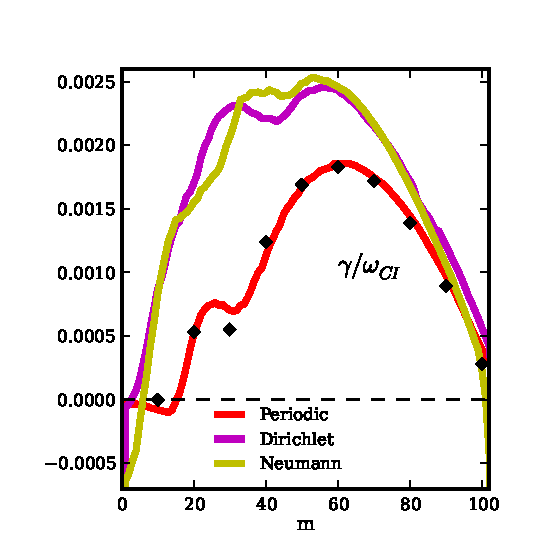
\includegraphics[]{lin_dw_gamma}}
\caption{Linear drift wave growth rates and axial structures}
\label{lin_dw_gamma}
\end{figure}

The LAPD equation set (Eqs.~\ref{ni_eq}-\ref{te_eq}) supports such drift waves, which are unstable with the parameters and profiles used in the simulations. 
The growth rate as a function of the azimuthal
wavenumber $m$ is shown in Fig.~\ref{lin_dw_gamma} a) for the LAPD parameters in Table~\ref{parameter_table} and profiles in Fig.~\ref{equilibrium_profiles}. The growth rates are found by simulating
the linearized version of Eqs.~\ref{ni_eq}-\ref{te_eq} in BOUT++ with the three different simple axial boundary conditions: periodic, zero-value (Dirichlet), and zero-derivative (Neumann). 
The linear equations simply omit the advective nonlinearities and the source terms, though the source terms have no affect on any of the linear modes besides $m=0$ modes. The simulations are run
for long enough so that the fastest growing modes can dominate the dynamics.

The solid curves in Fig.~\ref{lin_dw_gamma} are calculated from the simulation results using the formula, $\gamma_m = \pdiff{E_m}{t}/(2 E_m)$ where $E_m$ is the energy of the fastest
growing linear eigenmode with azimuthal mode number $m$.
The energy is defined in Chapter~\ref{c_en_formalism}. The details of obtaining $\gamma_m$ are explained in that chapter, but for now, it is sufficient to state that this procedure calculates
$\gamma_m$ at a particular time using only the structures of the fluctuating quantities: $N, \phi, \vpe, {\rm and } T_e$. An alternative way to calculate $\gamma_m$ is to use BOUT++'s Fourier
filtering capabilities and run many simulations where each one filters out a different azimuthal mode. Then, I take the log of the envelope of one or several of the fluctuating quantities
and calculate the slope of the line, which gives the growth rate for each particular simulation. This procedure uses the time signal of the fluctuations rather than their spatial structure to
calculate the growth rate, thus providing a check on the first method. 
The results using this alternative method for the periodic case are shown with the black diamonds in Fig.~\ref{lin_dw_gamma} a), which agree well with the curve calculated using the 
alternative energetic structure-based calculation. I do this check with all of the simulations to ensure consistency. This second method is more time consuming, so I only sample a few values of $m$.
Furthermore, it's difficult to get growth rates when $\gamma_m < 0$ using this second method.

The difference in the growth rate curves with the different boundary conditions is due to the different $k_\para = \frac{2 \pi n}{L_\para}$ where $n$ is the axial mode number. The periodic simulation
restricts $n$ to integer values, while the Dirichlet and Neumann simulations allow for any fractional $n$. The largest growth rate occurs for $n \sim 1/2$. The Dirichlet and Neumann axial structures
for the most unstable $m$ mode, shown in Fig.~\ref{lin_dw_gamma} b), reflect this. The periodic simulation, which has $n=1$ structure, has a smaller growth rate, especially at low $m$. Note that in
Fig.~\ref{lin_dw_gamma} b), the axial boundaries are not plotted. For instance, the zero-valued boundaries for the Dirichlet simulation are not shown. Also, the axial structures are taken at one
random point in the $r-\theta$ plane and at one time point, and are normalized to their maximum value.

\subsection{Conducting Wall Mode}
\label{ss_cwm}

\begin{figure}[!ht]
\centerline{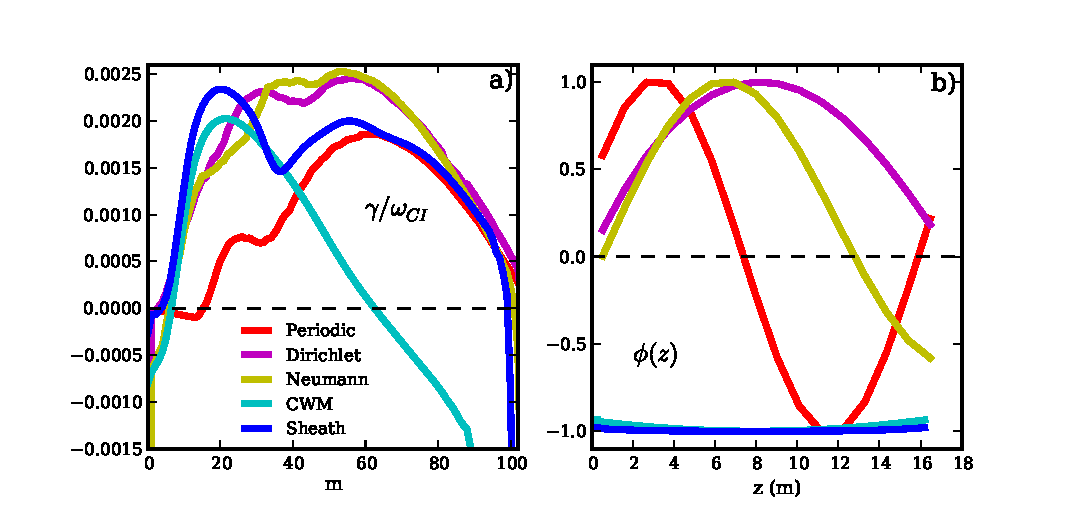
\includegraphics[]{lin_all_gamma}}
\caption{Linear conducting wall mode growth rates and axial structures}
\label{lin_all_gamma}
\end{figure}


I now consider the linear instability that can exist in a plasma bounded by two conducting walls on the boundaries where the magnetic field lines terminate
(the axial boundaries)~\cite{berk1991,berk1993,xu1993}.
The instability is actually of the drift wave variety, but unlike the drift waves discussed above, the pressure-potential coupling mechanism is through the sheath boundary response
rather than through the adiabatic response. The Bohm sheath boundary conditions that were derived in Sec.~\ref{ss_bs_bc} can provide this coupling. 
As already noted, these boundary conditions are not necessarily the correct ones
for LAPD, but are somewhat idealized. Yet, it is still academically instructive to apply such an idealized boundary condition to LAPD because it creates this new linear instability, which
can be used to test the robustness of LAPD's nonlinear instability.

The conducting wall mode (CWM) instability in the case considered here is purely an electron temperature gradient instability, although other types of gradients can cause it~\cite{berk1993}.
Electron temperature fluctuations are advected by electrostatic potential fluctuations and feed off the equilibrium electron temperature gradient as in the case of the thermal drift waves.
However, in contrast to the thermal drift waves, the coupling between the temperature and potential fluctuations comes through the sheath boundary condition rather than through the adiabatic
response. Furthermore, the CWM can have (nearly) $k_\para = 0$ flute-like behavior. The coupling mechanism is as follows: an electron temperature perturbation -- say a
positive constant fluctuation along a small flux tube -- increases the sound speed and the electron thermal speed on the flux tube. 
Since the ions must enter the Bohm sheath at the sound speed by being accelerated
by a parallel electric field, the temperature increase must coincide with an increase in the parallel potential gradient as derived in Eq.~\ref{sheath_bc}. Additionally, the increased
electron thermal speed causes an increase in the floating potential along the flux tube. These serve to couple the electron temperature to the potential.

The CWM can be isolated from the normal drift waves by removing the adiabatic response from the full LAPD equation set, and of course using the Bohm sheath boundary condition of Eq.~\ref{sheath_bc}.
Removal of the adiabatic response in this case means removal of the $\gradpar p_e$ and the $0.71 \gradpar T_e$ terms in the parallel momentum equation (Eq.~\ref{ve_eq}). This causes the 
density fluctuation $N$ to become a passive scalar, so Eq.~\ref{ni_eq} can be removed as well with no consequence. So the isolated linear CWM equations are:

\beqar
\label{ve_eq_cwm}
\pdt \vpe = \fmie \gradpar \phi - \nue \vpe, \\
\label{rho_eq_cwm}
\pdt \varpi = - N_0 \gradpar \vpe - \nuin \varpi + \mu_\phi \gradperp^2 \varpi, \\
\label{te_eq_cwm}
\pdt T_e = - {\mathbf v_E} \cdot \grad T_{e0} + \frac{2}{3 N_0} \kpe \gradpar^2 T_e  - \frac{2 m_e}{m_i} \nue T_e  + \mu_T \gradperp^2 T_e,
\eeqar

The CWM growth rate curve is shown in Fig.~\ref{lin_all_gamma} a). The CWM is most unstable at values of $m \sim 20$, which is much lower than the $m \sim 60$ values of the drift waves.
Furthermore, the CWM maximum growth rate is about equal to the drift wave growth rates. And from Fig.~\ref{lin_all_gamma} b), the CWM axial structure is flute-like ($k_\para \simeq 0$). 
Finally, the growth rate curve of the full set of equations along with the sheath boundary condition is shown in this figure as the curve labeled ``sheath.'' This set of equations contains
the drift wave and CWM instabilities. From both Figs.~\ref{lin_all_gamma} a) and b), it is clear that the sheath simulation is dominated by the CWM at $m \leq 20$, which in fact is where
the growth rate is maximum. At $m \geq 40$, the drift waves dominate.


\section{LAPD Turbulence: A Visual Examination}
\label{s_vis_exam}

\begin{figure}[!ht]
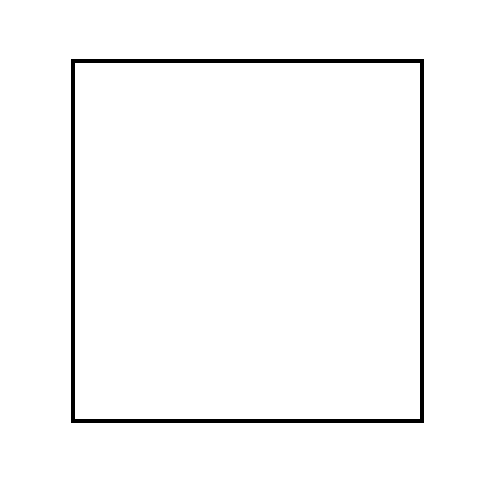
\includegraphics[]{empty_box}
\centering
\caption{3D turbulent simulation animation}
\label{3D_turb_anim}
\end{figure}


When I simulate the full LAPD equation set with the advective nonlinearities and source terms, I find that the simulation develops into a turbulent state. To start the simulation,
I initialize each fluctuation quantity ($N, \phi, \vpe, {\rm and } \ T_e$) with a small random 3D spatial structure. The structure evolves and a coherent structure emerges (the fastest
growing linear eigenvector), which grows exponentially in time. Once the normalized fluctuations reach values on the order of $0.01-0.1$, they saturate and appear to be turbulent.
A 3D animation of the density fluctuation $N$ is shown in Fig.~\ref{3D_turb_anim}. The animation shows a $1/8$th wedge of the simulated annulus to make the axial extent of the annulus visible.
The animation begins right before the fastest growing mode structure becomes dominant. The fastest growing mode dominates the structure for some time, where there is a clear coherent
wave structure that simply propagates in the electron diamagnetic drift direction. This stage is called the linear stage since the linear terms in the equations dominate the evolution.
Note that the axial structure in the linear stage has a finite wavelength about half of the length of the animation domain. The axial boundary conditions used here (Neumann) allow for
such a structure.

Soon, the coherent eigenmode structure, which has been growing in magnitude, saturates and transitions to a turbulent-looking state that I call the turbulent stage.
The evolution of the RMS fluctuation amplitude of the density and potential is shown in Fig.~\ref{rms_evolution} a). The potential is separated into a flux-surface-averaged component $\phi_{fs}$
and the remainder $\phi-\phi_{fs}$. $\phi_{fs}$ quantifies the amplitude in the zonal flow, which appears in Fig.~\ref{rms_evolution} a) to possibly have some role in the initial saturation, but
has a relatively small magnitude in the turbulent stage.
For all the fluctuations, the exponential growth period during the linear stage is followed by saturation corresponding to the
visual change from coherent to turbulent spatial structures in the animation. 
Upon transition to the turbulent stage, I notice in the animation that there is also a qualitative change in the axial
mode structure. The axial structures elongate, looking more flute-like than in the linear stage. I confirm this by taking the axial Fourier transform of the density fluctuations and plotting
the RMS values of the different axial mode numbers in Fig.~\ref{rms_evolution} b). The linear stage is dominated by the $n=1$ Fourier component, while the turbulent stage is dominated
by the $n=0$ flute mode component. I found this to be an interesting and unexpected transition when I first identified it. There is not only the expected bifurcation from linear waves to turbulence,
but also the unexpected bifurcation from linear drift wave structures to turblent flute-like structures. I will discuss why this is unexpected in the upcoming chapters, and I will show in detail
what causes it. But take note that this is a key finding. This $n=0$ dominance in the turbulent stage is the main subject of the remaining chapters.


\begin{figure}[!ht]
\centerline{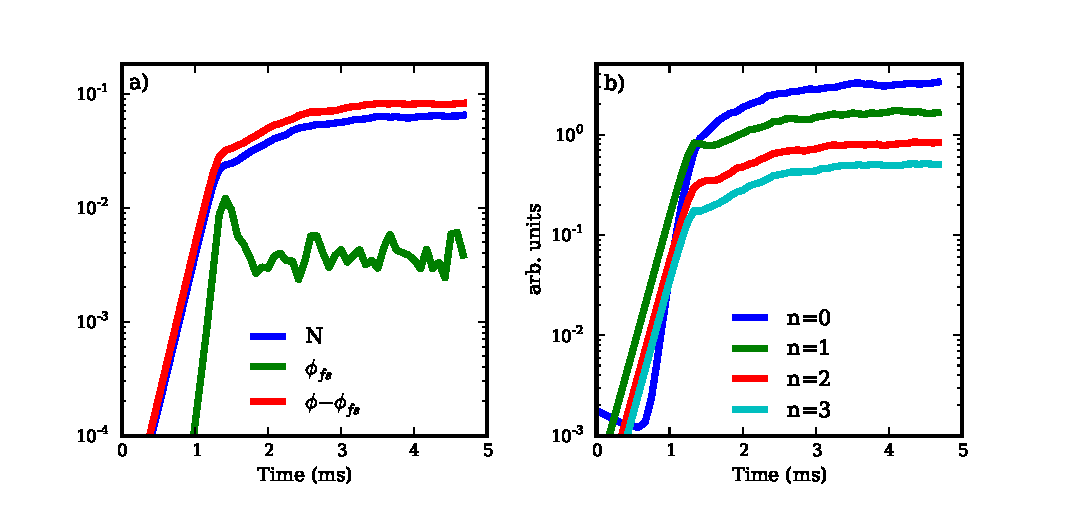
\includegraphics[]{rms_evolution}}
\caption{RMS time evolution of fluctuations and axial mode numbers}
\label{rms_evolution}
\end{figure}


However, before I jump into the analysis of the $n=0$ mode dominance, I continue to look at simple and common turbulence analysis techniques to describe the nature of the turbulence
and to validate the simulations.
Continuing on with the visual examination, I show one visual comparison between the simulation and experiment. For the experimental visual, I use a processed
fast camera movie. The camera records the light intensity given off by the plasma. The light is primarily due to line radiation of the helium atoms and ions. It should be some function
of plasma density, neutral density, and plasma temperature. Noting that the comparison is certainly not exact, I show the experimental camera data next to corresponding simulation
data of the density $N$ signal during the turbulent stage. This is shown in Fig.~\ref{sim_v_exp_anim}. 
The animations cover the same spatial domain and last for equal time intervals (about 2 ms). Both are simply fluctuation
data with the time-independent background not included (subtracted out from the camera data). 

Visual comparisons like this are certainly not quantitative, and at best this comparison
reveals that both simulatin and experiment appear turbulent and contain similarly sized spatial structures and similar time scales. The camera data can be a valuable tool since it provides
so much simultaneous spatial data -- something that is difficult to do with probes. Nevertheless, I do not proceed here with detailed statistical analysis of the camera data or any
quantitative comparisons between the camera and simulation. This work is left for future studies. Rather, I now focus on statistical analysis of the simulation data, and compare it to
experimental Langmuir probe data when possible.


\begin{figure}[!ht]
\centerline{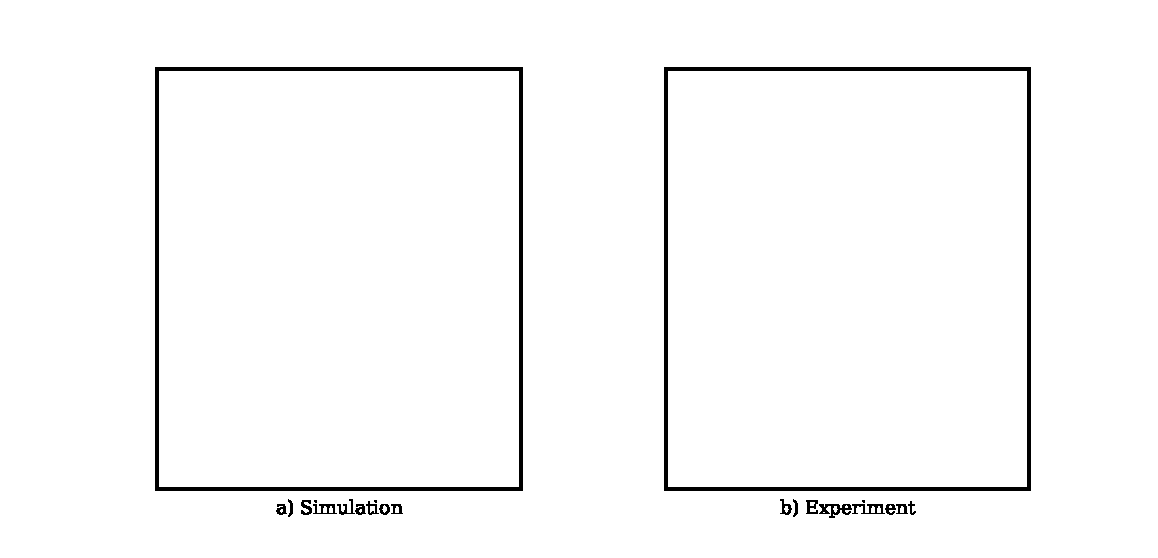
\includegraphics[]{2empty_box}}
\caption{Turbulent movies}
\label{sim_v_exp_anim}
\end{figure}


\section{LAPD Turbulence: A Statistical Examination}
\label{s_stat_exam}

Dynamical systems are often described statistically using such tools as spectra, pdfs, and spatial and temporal correlations. This is probably the most common way to describe stochastic systems,
but it is also common to describe chaotic systems this way as well. The goal is to be able to characterize the fluctuations. At the very least, this provides a good way to compare simulations
to the experiment in order to validate the simulation model. In a stronger way, different theories of turbulence make different predictions regarding statistics, making such a characterization
important for confirming or disreputing theories. In this section, I focus mostly on simple comparisons between simulation and experiment, but I also point out some characteristics that are
for certain theoretical predictions.

Now before I proceed with statistical data comparisons to qualify and quantify the agreement between the simulations and experiment, I must first explain how I can extract
equivalent information from the simulations and experiment. In general, this hinges upon experimental measurement theory.

\subsection{Experimental Probe Data}
\label{ss_probe_data}

There are many different kinds of experimental measurements, but I focus here only on Langmuir probe measurements. The Langmuir probes in LAPD generally provide time series data although
I do have some two-probe data that provides certain spatial information. Langmuir probes do not directly measure any of the independent state or flux variables of the simulation 
($N, \phi, \vpe, T_e$), but they can measure quantities that are functions of these variables. The probes are biased to a known potential (with respect to a reference like the cathode potential),
and the current they draw from the plasma is measured. As long as the probes are biased sufficiently below the plasma potential so as to repel most electrons, 
they develop sheaths around them in the same way as the conducting plates considered in Sec.~\ref{ss_bs_bc}. The ion current to the probe is~\cite{hutchinson2002}

\beq
\label{probe_ion_current}
I_i \sim \frac{1}{2} e A_s n c_s
\eeq

where $A_s$ is the sheath area, approximately equal to the probe area, and the factor of $\frac{1}{2} n$ is the reduction of density at the sheath edge compared to the main plasma.
The probe may be biased negatively enough so that all electrons are repelled. The current collected is just that of Eq.~\ref{probe_ion_current}, called the ion saturation current.
As the probe voltage is swept positively from this point, more electrons are collected. The total current to the probe then takes the form~\cite{hutchinson2002}

\beq
\label{probe_current}
I = e A_s n c_s \left[\frac{1}{2} - \left(\frac{m_i}{2 \pi m_e} \right)^{1/2}  e^{e V_p/T_e} \right],
\eeq

where $V_p$ (which is negative) is the potential of the probe with respect to the plasma potential. When $I=0$, the probe potential is at the floating potential: 
$\frac{e (V_f - \phi)}{T_e} = \frac{1}{2} {\rm ln} \left(\frac{\pi m_e}{2 m_i}\right)$. The temperature can be obtained by sweeping the probe potential to get $\pdiff{I}{V_p}$, 
which is an exponential function of $V_p$.
So the logarithm of this function produces a straight line. Then, the temperature is:

\beq
\label{probe_temp}
T_e = e (I - I_i)/\pdiff{I}{V_p}.
\eeq

Now the sweeping process is too slow to obtain temperature fluctuations. It's best used to obtain the equilibrium temperature profile. Since a single Langmuir probe doesn't give
temperature fluctuations, it's impossible to find the exact density and potential fluctuations, $N$ and $\phi$. The probes only produce $I_{sat}$ and $V_f$ fluctuation data.
Nevertheless, the simulations produce $N, \phi$, and $T_e$
fluctuations, which I can use to calculate the $I_{sat}$ and $V_f$ simulation values using the relations: $I_{sat} = \frac{1}{2} e A_s n c_s$ and
$V_f = \phi + \frac{T_e}{2 e} {\rm ln} \left(\frac{\pi m_e}{2 m_i}\right)$. So rather than manipulating probe data to find the experimental $N$ and $\phi$ fluctuations, I can
use the simulation data to calculate experimentally-accessable quantities. The derived simulation quantities are called synthetic diagnostics. 
Synthetic diagnostics are model-dependent and they bind together some of the fundamental
underlying data. For instance, two measurements ($I_{sat}$ and $V_f$) comprise three fundamental state variables ($N, \phi,$ and $T_e$), so the synthetic diagnostics bind the temperature fluctuations
to the density and potential fluctuations. Nevertheless, synthetic diagnostics provide a way to make
apples-to-apples comparisons between simulation and experimental data.


\begin{figure}[!ht]
\centerline{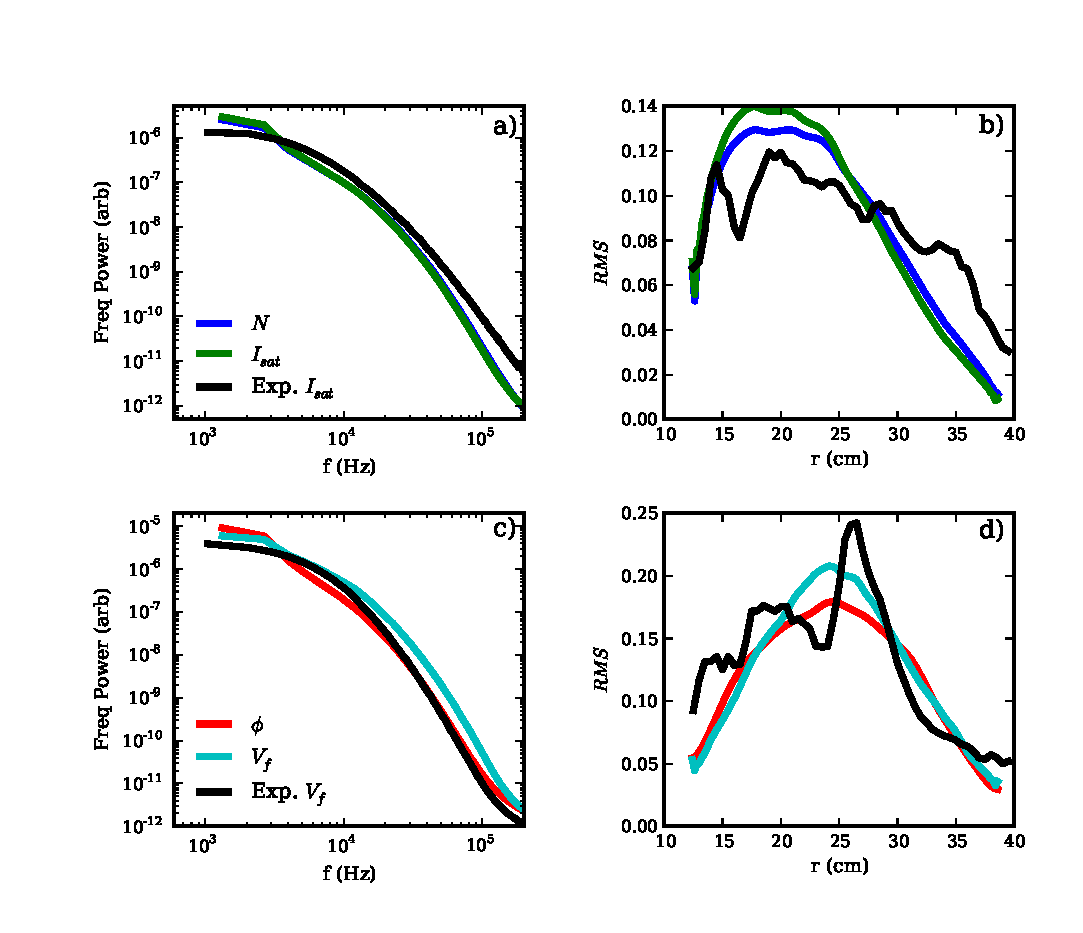
\includegraphics[]{isat_vf_statistics}}
\caption{$I_{sat}$ and $V_f$ statistical data}
\label{isat_vf_statistics}
\end{figure}

I show in Fig.~\ref{isat_vf_statistics}, a statistical comparison between $I_{sat}$ and $V_f$ fluctuations from simulation and experiment. The simulation uses the full nonlinear equation
set along with Bohm sheath axial boundary conditions. I also show simulation statistics for $N$ and $\phi$ fluctuations so that they may be compared to the simulation statistics of the synthetic
$I_{sat}$ and $V_f$ respectively. Figs.~\ref{isat_vf_statistics} a) and b) compare the frequency spectra and radial RMS amplitudes of experimental and simulation $I_{sat}$ 
fluctuations along with $N$ fluctuations from the simulation. Figs.~\ref{isat_vf_statistics} c) and d) compare the same statistical properties, but this time of $V_f$ 
fluctuations along with $\phi$ fluctuations from the simulation. The $I_{sat}$ fluctuations from the simulation have nearly identical statistical properties as the $N$ fluctuations
because $I_{sat}$ is proportional to density but only weakly dependent on temperature (square root dependence). $V_f$ fluctuations are also somewhat similar to $\phi$ fluctuations,
but to a lesser degree due to the large dependence of $T_e$ on $V_f$. Furthermore, the simulation and experiment have very similar statistical properties, which I expand upon below.

\subsection{Statistical Density Comparisons}
\label{ss_stat_dens_comps}

\begin{figure}[!ht]
\centerline{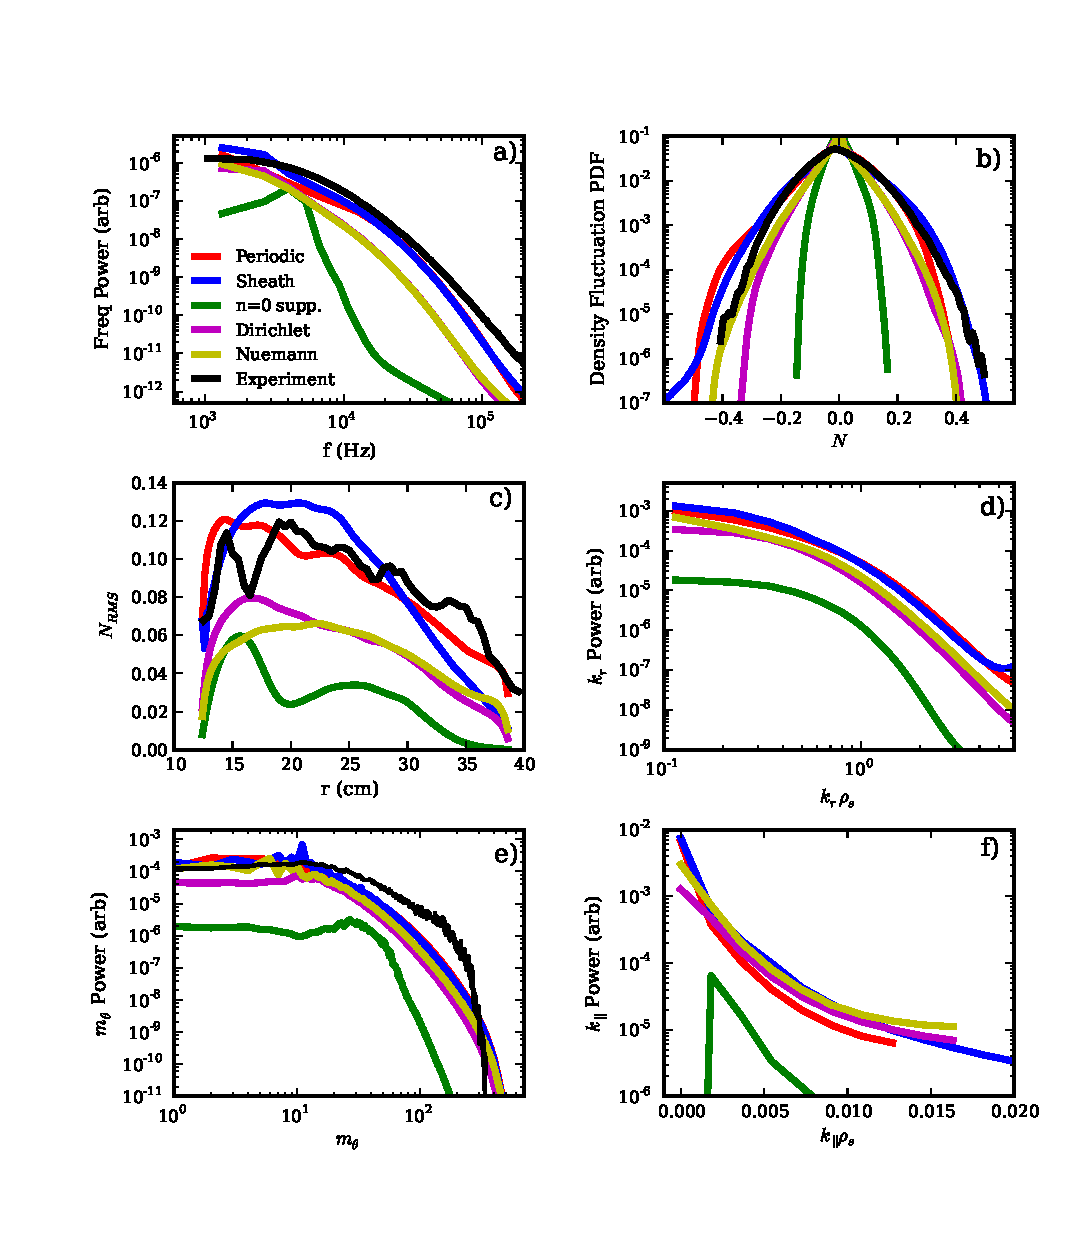
\includegraphics[]{n_statistics}}
\caption{Density statistics}
\label{n_statistics}
\end{figure}


A comparison of statistical properties of the experimental and simulation density fluctuations is shown in Fig.~\ref{n_statistics}. I actually compare the $N$ fluctuations for the simulations
to the $I_{sat}$ fluctuations of the experiment, but as seen in Fig.~\ref{isat_vf_statistics}, $I_{sat}$ and $N$ statistics are nearly identical.
Fig.~\ref{n_statistics} contains results from five different simulations
that all use the full nonlinear LAPD equation set (Eqs.~\ref{ni_eq}-\ref{te_eq}) but differ in the axial boundary conditions as follows:
1) Periodic -- uses periodic axial boundary conditions. 2) Sheath -- uses Bohm sheath boundary conditions (Eq.~\ref{sheath_bc}). 3) $n=0$ suppressed -- uses axial boundary conditions,
however, the axial average ($k_\para$ or $n = 0$) density, temperature, and potential fluctuation components are artifically removed from the simulation. 4) Dirichlet -- uses zero-value axial
boundary conditions. 5) Neumann -- uses zero-first-derivative axial boundary conditions. I will discuss the $n=0$ suppressed simulation more in Chapter~\ref{c_nlin_periodic}, but for
now it is sufficient to say that this simulation does not contain the nonlinear instability and is thus a control case by which to compare the others. It still contains the same
linear instabilities as the Periodic simulation, however.

Fig.~\ref{n_statistics} a) shows the frequency power spectrum of the density fluctuations. I use a sliding Hamming window on the time series data and take the FFT, then take a volume
average from 15 to 35 cm to get each simulation curve. I use the same technique for the experimental density fluctuation data, except I only have probe data at one location in the
$\theta-z$ plane. The axial location is near the center of the machine. I plot the frequency spectrum in a log-log format to emphasize the low-frequency comparison, which is where most of the
power is located, but I also show the spectrum in a log-linear format in Fig.~\ref{lorentzians}, and discuss this more later.
Fig.~\ref{n_statistics} b) shows the probability distribution function (PDF) of the density fluctuations, while I provide the first four PDF moments in Table~\ref{pdf_moments}, which characterize
the shape of the PDFs, and most importantly their non-Gaussianity.
Fig.~\ref{n_statistics} c) shows the RMS amplitude of the density fluctuations as a function of radius, while Fig.~\ref{n_statistics} d) plots the radial $k_r$ power spectrum of the simulations.
I don't have experimental radial spectra data, which requires multiple probes at different radii. Fig.~\ref{n_statistics} e) is the azimuthal $m_\theta$ power spectra. 
Two probes separated azimuthally are used to obtain the experimental spectra. Finally Fig.~\ref{n_statistics} f) is the axial $k_\para$ spectra, and I don't have experimental axial spectra due
to the difficulty of aligning two probes along a field line a significant distance from each other, which is required because of the long axial wavelengths of the modes.

Fig.~\ref{n_statistics} and Table~\ref{pdf_moments} contain a lot of information about the simulations and experiment. 
The first obvious result is that the $n=0$ suppressed simulation is statistically much different
than all of the other simulations and the experiment. The density fluctuations of this simulation are a factor of 2-3 lower than that of the other simulations and the experiment.
Furthermore, this simulation has peaks in the frequency, $m_\theta$, and $k_\para$ spectra that are unique. The frequency and $m_\theta$ peaks are inconsistent with the experiment. 
Its spatial spectra peak at
$m_\theta \sim 30$ and $k_\para \rho_s \sim 0.002 \rightarrow n = 1$, which is somewhat consistent with the linear growth rate spectra of Fig.~\ref{lin_dw_gamma}, although the $m_\theta$
peak location is somewhat less than the maximum linear growth rate value of $m_\theta$, which is around 60 when the axial boundaries are periodic. 
This differs significantly from all of the other simulations and the experiment which have peaks at $m_\theta \sim 10$ (if they peak at all).
And again, as was clear from Fig.~\ref{rms_evolution} b), all of the other simulations are strongly dominated by $n=0$ axial mode numbers, which will be explained
in the upcoming chapters as due to the nonlinear instability.

Moreover, all of the simulations other than the $n=0$ suppressed simulation have qualitatively and semi-quantitatively similar statistical properties, which are also consistent with the
statistical properties of the experiment. For instance, they all possess broadband
frequency and wavenumber spectra of the same general shape, they all have similarly shaped radial fluctuation amplitudes,
and the fluctuations all have kurtosis greater than 3, meaning that the tails of the PDFs are larger than for a Gaussian distribution.
I note that on a quantitative level,
the Dirichlet and Neumann simulations have fluctuation levels about 1.5 times less than the Periodic and Sheath simulations. I don't fully understand the reason for this, but note
that the axial wavenumber spectra in Fig.~\ref{n_statistics} f) are shallower for the Dirichlet and Neumann simulations. This certainly affects the energy injection and energy
dissipation, as will be seen in the following chapters. Nevertheless, even though their fluctuation levels are too low,
I don't claim that the Dirichlet and Neumann simulations are less consistent with the experiment than the
Periodic and Sheath simulations. The reason is that I have a free parameter, namely the artificial
diffusion coefficient, which affects the overall fluctuation level without significantly affecting the shapes of the spectra. I tuned this parameter to be 
$1.25 \times 10^{-3}$ (see Chapter~\ref{c_lapd_sim})
to match the fluctuation level of the Periodic simulation with experiment. Had I tuned this parameter with the Dirichlet or Neumann simulations in mind, it would seem that
the Periodic and Sheath simulations had fluctuation levels too large. So, in fact, all four of these simulations are qualitatively consistent with the experiment, and they are also
quantitatively consistent with the caveat that the quantitative match is caused by tuning a single free parameter. I don't provide any error analysis to quantify the agreement
between simulation and experiment, but rather just use an eye test. The fact that several different statistical properties of several fields (see Fig.~\ref{isat_vf_statistics})
agree between simulation and experiment lends evidence to my claim that the simulation model is relatively well validated.

\begin{figure}[!ht]
\centerline{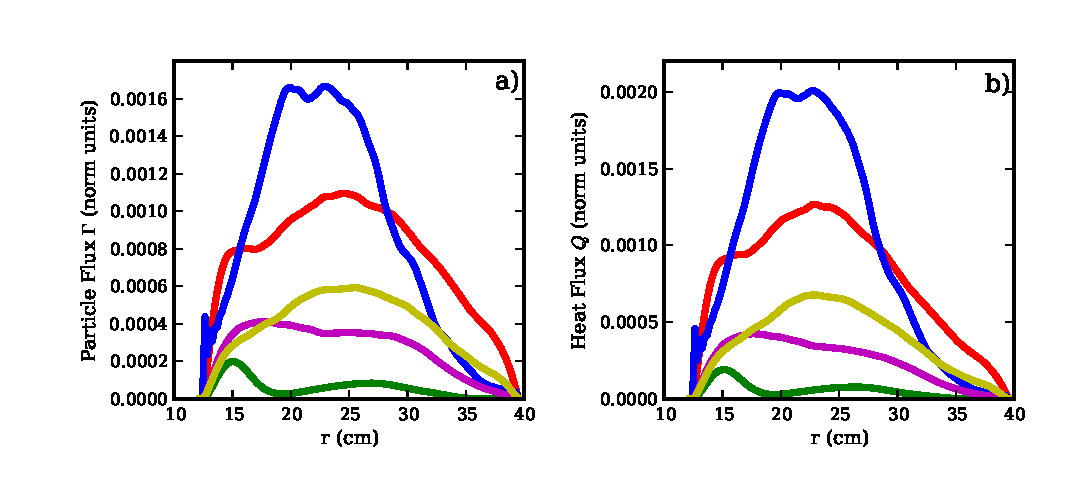
\includegraphics[]{radial_flux}}
\caption{Radial particle and heat flux}
\label{radial_flux}
\end{figure}

Another statistical property that is of utmost importance is the radially convective flux (both particle and heat flux), which ultimately dominate the transport in turbulent magnetic
confinement devices. I show the particle flux, $\Gamma = \left< N v_r \right>$, and energy flux, $Q = \left< N T_e v_r \right>$, in Fig.~\ref{radial_flux}, where $V_r$ is the radial
${\bf E \times B}$ velocity due to the fluctuating potential. Although this transport is convective, many write the flux in terms of diffusion coefficients based on Fick's Law:
$\Gamma = - D \grad N_0$ and $Q = -N_0 \chi \grad T_{e0}$. For the largest fluxes in Fig.~\ref{radial_flux} -- those corresponding to the Sheath simulation -- the maximum diffusion coefficients
are $D_{max} \approx 5 \rm{m^2/s}$ and $\chi_{max} \approx 7 \times 10^{5} \rm{s^{-1}}$. For comparison, the Bohm diffusion coefficient for these simulations is $D_{Bohm} \approx 3 \rm{m^2/s}$.
So the transport in the simulations other than the $n=0$ suppressed simulation is consistent with the Bohm value.

\begin{figure}[!ht]
\centerline{\includegraphics[]{n_correlations}}
\caption{Spatial density correlations}
\label{n_correlation}
\end{figure}


\begin{figure}[!ht]
\centerline{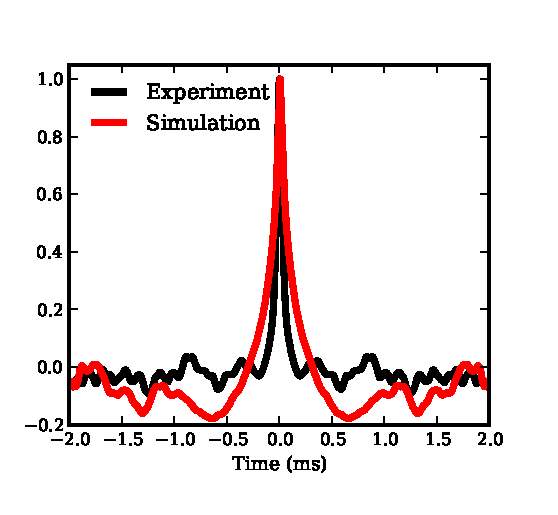
\includegraphics[]{autocorrelation}}
\caption{Temporal density autocorrelation}
\label{autocorrelation}
\end{figure}


Another statistical measurement that may be compared between simulation and experiment is the spatial and temporal correlation. Experimentally, the spatial correlation
can be done by fixing one probe at a certain
location and moving another probe around and measuring the correlation between the two $I_{sat}$ signals. The second probe can scan the $r-\theta$ plane at an axial location close
to the first probe. The results of the simulated spatial correlation compared to the experimental correlation are shown in Fig.~\ref{n_correlation}. For the simulation, I show only
the result from the Periodic simulation. The darkest red point, which
has a correlation value of 1 marks the location of the stationary probe. The black line is the $1/e$ contour, where the distance from the stationary probe to this contour is
the correlation length. The simulation correlation length of about 1 cm is about half of that of the experimental correlation length. Furthermore, neither have completely isotropic
structure, and their slight divergences from isotropy are not that similar. However, there is no complex mode structure or long extended correlations in either one.

As for the temporal correlation, this is easily done with a single stationary probe. I show the results of the experiment
and a simulation in Fig.~\ref{autocorrelation}, 
showing that the autocorrelations recede exponentially (confirmed by a semilog plot), with the simulation having a longer correlation time than the experiment. This is not
surprising given the visually longer lived structures in the simulation as seen in Fig.~\ref{sim_v_exp_anim}.



\begin{table}
\label{pdf_moments}
\setlength{\tabcolsep}{12pt}
\begin{tabular}{| p{2cm} || p{2cm} | p{2cm} | p{2cm} | p{2.2cm} |}
\hline 
Dataset & Mean $\quad \quad \overline{N}$ & STD $\quad \sigma^2 = \overline{N^2}$ & Skewness $S = \overline{N^3}/\sigma^3$ & Kurtosis $\quad K = \overline{N^4}/\sigma^4$ \\ \hline \hline
Periodic & $-3.2 \times 10^{-8}$ & $8.4 \times 10^{-3}$ & $-0.17$ & $3.9$ \\ \hline
Sheath  & $1.0 \times 10^{-4}$ & $9.5 \times 10^{-3}$ & $0.14$ & $3.9$ \\ \hline
$n=0 \quad$ suppressed & $-4.7 \times 10^{-6}$ & $9.6 \times 10^{-4}$ & $0.17$ & $4.5$ \\ \hline
Dirichlet & $6.2 \times 10^{-4}$ & $3.4 \times 10^{-3}$ & $0.18$ & $5.2$ \\ \hline
Neumann & $2.2 \times 10^{-5}$ & $3.5 \times 10^{-3}$ & $0.045$ & $5.8$ \\ \hline
Experiment & $-2.4 \times 10^{-6}$ & $8.2 \times 10^{-3}$ & $0.18$ & $3.5$ \\ \hline
\end{tabular}
\caption{PDF moments}
\end{table}
